% !TeX root = ../tfg.tex
% !TeX encoding = utf8

\chapter{Redes neuronales artificiales}
\label{chapter:ann}

Dentro de los distintos modelos de aprendizaje automático, nosotros trabajaremos
con redes neuronales artificiales. Para entender mejor su funcionamiento,
primero hablaremos de las neuronas biológicas y su inspiración en los modelos
artificiales.

\section{Neuronas biológicas}

Las neuronas biológicas son células especializadas del sistema nervioso que desempeñan
roles clave en la recepción, procesamiento y transmisión de señales
\cite{rosenblatt1958perceptron}. Estas células son fundamentales para la comunicación
neuronal, permitiendo el flujo de información a través de complejas redes en el
cerebro y otros componentes del sistema nervioso.

Las neuronas biológicas están compuestas por tres partes principales: el \textbf{soma},
que es el cuerpo celular conteniendo el núcleo y orgánulos celulares; las
\textbf{dendritas}, extensiones que reciben señales de otras neuronas; y el \textbf{axón},
una prolongación especializada que conduce los potenciales de acción desde el soma
hasta las terminaciones sinápticas. Estas terminaciones sinápticas se encuentran
en las sinapsis, donde se produce la transmisión de señales a otras neuronas o tejidos
(\autoref{fig:neurona}).

\begin{figure}[H]
	\centering
	\includegraphics[width=100mm, scale=0.5]{img/neuron.png}
	\caption{Representación esquemática de una neurona biológica, mostrando el soma,
		las dendritas y el axón. Fuente \href{http://creativecommons.org/licenses/by-sa/3.0/}{User:Dhp1080,
			CC BY-SA 3.0}, via Wikimedia Commons.}
	\label{fig:neurona}
\end{figure}

Esta compleja red de conexiones y la regulación electroquímica hacen que las
neuronas biológicas sean fundamentales para coordinar y ejecutar numerosas
funciones, desde simples reflejos hasta procesos cognitivos avanzados.

\section{Redes neuronales artificiales}

Las \textbf{neuronas artificiales} se inspiran en las neuronas biológicas en el sentido
de que ambas tienen la capacidad de recibir, procesar y transmitir señales. En el
caso de las neuronas artificiales, estas reciben señales de otras neuronas
dentro de una red y las procesan mediante una combinación lineal de una matriz
de \textbf{pesos} ajustables $\mathbf{W}$ y un vector de \textbf{sesgo} o
\textbf{\textit{bias}} $\mathbf{b}$. Durante el entrenamiento de la red, estos parámetros
se refinan para optimizar el rendimiento de la red en tareas específicas como clasificación
o regresión. Cada neurona artificial aplica una función escalar denominada
\textbf{función de activación} $\theta: \mathbb{R}^{m} \to \mathbb{R}$, que
transforma la combinación lineal de sus entradas:

\[
f(\mathbf{x}, \mathbf{W}, \mathbf{b}) = \theta(\mathbf{W}\mathbf{x}+ \mathbf{b}
), \quad \forall \mathbf{x}\in \mathbb{R}^{d}, \mathbf{W}\in \mathbb{R}^{m
	\times d}, \mathbf{b}\in \mathbb{R}^{m}.
\]

Aquí, $d$ es la dimensión de entrada y $m$ es el número de neuronas en la capa.

Estas neuronas se agrupan en \textbf{capas} dentro de una \textbf{red neuronal
	artificial} (ANN). La estructura de la red se define por su \textbf{profundidad},
que corresponde al número de capas ocultas, y su \textbf{anchura}, que se
refiere al número de neuronas en cada capa.

\begin{figure}
	\centering
	\def\layersep{2.5cm}
	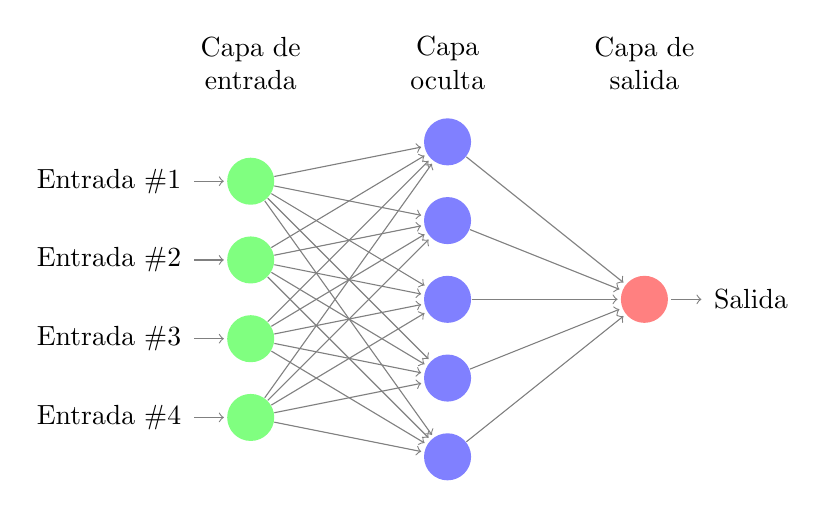
\begin{tikzpicture}[shorten >=1pt, ->, draw=black!50, node distance=\layersep]
		\tikzstyle{every pin edge}
		=[<-,shorten <=1pt]
		\tikzstyle{neuron}
		=[circle,fill=black!25,minimum size=17pt,inner sep=0pt]
		\tikzstyle{input neuron}
		=[neuron, fill=green!50];
		\tikzstyle{output neuron}
		=[neuron, fill=red!50];
		\tikzstyle{hidden neuron}
		=[neuron, fill=blue!50];
		\tikzstyle{annot}
		= [text width=4em, text centered]
		
		% Draw the input layer nodes
		\foreach \name / \y in {1,...,4}
		% This is the same as writing \foreach \name / \y in {1/1,2/2,3/3,4/4}
		\node[input neuron, pin=left:Entrada \#\y] (I-\name) at (0,-\y) {};
		
		% Draw the hidden layer nodes
		\foreach \name / \y in {1,...,5} \path[yshift=0.5cm] node[hidden neuron] (H-\name)
		at (\layersep,-\y cm) {};
		
		% Draw the output layer node
		\node[output neuron,pin={[pin edge={->}]right:Salida}, right of=H-3] (O) {};
		
		% Connect every node in the input layer with every node in the
		% hidden layer.
		\foreach \source in {1,...,4} \foreach \dest in {1,...,5} \path (I-\source) edge
		(H-\dest);
		
		% Connect every node in the hidden layer with the output layer
		\foreach \source in {1,...,5} \path (H-\source) edge (O);
		
		% Annotate the layers
		\node[annot,above of=H-1, node distance=1cm] (hl) {Capa oculta}; \node[annot,left
		of=hl] {Capa de entrada}; \node[annot,right of=hl] {Capa de salida};
	\end{tikzpicture}
	\caption{Estructura de una FNN. Muestra una red neuronal hacia adelante con tres
		tipos de capas: entrada (verde), oculta (azul), y salida (rojo). Cada neurona de
		la capa de entrada está conectada a todas las neuronas en la capa oculta,
		demostrando un ejemplo de capas totalmente conectadas.}
	\label{fig:fnn}
\end{figure}

En el caso de las \textbf{redes neuronales hacia adelante} o \textbf{\textit{feedforward
		networks}} (FNNs), la red está compuesta por varias capas cuyas neuronas
solamente están conectadas a neuronas en capas posteriores (\autoref{fig:fnn}). En
el caso donde todas las salidas de una capa están conectadas a todas las neuronas
de la siguiente capa se les conoce como \textbf{capas totalmente conectadas} o
\textbf{\textit{fully connected layers}} (FC). Las funciones de cada capa en una
FNN pueden describirse como:

\[
f_{j}(\mathbf{x}) = \theta \left( \mathbf{W}_{j} \mathbf{x}+ \mathbf{b}_{j} \right
),
\]

donde $\mathbf{W}_{j}$ es la matriz de pesos y $\mathbf{b}_{j}$ es el vector de sesgo
para la capa $j$. Estos elementos son fundamentales para determinar cómo se
transforman las entradas en salidas que serán utilizadas por la siguiente capa. La
estructura funcional de las FNNs se describe entonces mediante la composición de
estas funciones organizadas en capas:

\[
\nu = s \circ f_{l} \circ f_{l-1}\circ \ldots \circ f_{2} \circ f_{1}(\mathbf{x}
),
\]

donde $l$ denota el número total de capas. La última capa de la red utiliza una función
de activación $s$, que convierte la salida de la capa final en uno o varios
valores en función de la tarea designada a la red. Esta función de salida es crítica
para aplicaciones como clasificación, donde el resultado necesita expresarse
como una probabilidad, o para regresión, donde se ajusta a un rango específico.

\section{Funciones de activación}

Las funciones de activación son de gran importancia en la arquitectura de las ANNs,
ya que introducen no linealidades en el modelo, permitiendo a la red aprender y modelar
relaciones complejas en los datos. Sin estas funciones, la red no podría resolver
tareas más complejas que una simple regresión lineal.

Anteriormente, hemos definido las funciones de activación en un contexto
vectorial, aplicando una única transformación a todas las entradas procedentes de
la capa anterior. Sin embargo, en la práctica es habitual emplear una función de
activación escalar $\theta : \mathbb{R}\rightarrow I$, donde $I$ es un intervalo
específico, de forma que se aplica componente a componente a cada combinación lineal
de entrada.

Una de las funciones de activación más antiguas es la \textbf{sigmoide}, que se define
como:
\begin{equation}
	\theta(z) = \frac{1}{1 + e^{-z}},
\end{equation}
donde $\theta : \mathbb{R}\to [0,1]$ y $z$ es la combinación lineal de entradas,
pesos y sesgo de la neurona. La función sigmoide transforma los valores de
entrada a un rango entre $0$ y $1$, modelando de esta forma probabilidades.
Aunque su uso ha disminuido en redes profundas debido al problema del \textbf{desvanecimiento
	del gradiente}, problema que consiste en que los gradientes van disminuyendo
progresivamente conforme profundizan en las capas de la red, impidiendo así su actualización.
A pesar de ello, sigue siendo relevante en la capa de salida de ANNs para clasificación
binaria.

La función \textbf{Softmax} es una generalización de la sigmoide para múltiples
clases y se define para un vector $z \in \mathbb{R}^{K}$ como:
\begin{equation}
	\theta(z)_{i} = \frac{e^{z_i}}{\sum_{k=1}^{K} e^{z_k}}\quad \text{para }i = 1,
	\ldots, K,
\end{equation}
donde $\theta : \mathbb{R}^{K} \to [0,1]^{K}$. Cada componente de la salida, $\theta
(z)_{i}$, representa la probabilidad de que la entrada pertenezca a la clase $i$,
y se utiliza principalmente en la capa de salida de las redes neuronales para tareas
de clasificación multiclase.

La \textbf{tangente hiperbólica} ($\tanh$), que se define como:
\begin{equation}
	\theta(z) = \tanh(z) = \frac{2}{1 + e^{-2z}}- 1,
\end{equation}
donde $\theta : \mathbb{R}\to [-1,1]$, es preferida sobre la sigmoide en algunos
escenarios por su salida centrada en cero, que facilita la optimización durante
el entrenamiento. Aunque también sufre del problema de desvanecimiento de gradiente,
su uso en capas ocultas es bastante frecuente.

La \textbf{\textit{Rectified Linear Unit}} (ReLU), definida como:
\begin{equation}
	\theta(z) = \max(0, z),
\end{equation}
donde $\theta : \mathbb{R}\to [0, \infty)$, es la más utilizada en aprendizaje
profundo por su simplicidad y eficiencia computacional. ReLU se utiliza generalmente
en capas ocultas, pero no es adecuada para la capa de salida en tareas de
clasificación debido a su rango no acotado. Además, ReLU sufre de un problema de
\enquote{\textbf{muerte de neuronas}} o \enquote{\textbf{\textit{dying ReLU}}}, que
sucede cuando los valores de entrada son menores o iguales a cero. Debido a que
la salida de ReLU es cero para estos valores, los gradientes también son cero durante
la retropropagación. Como resultado, estas neuronas dejan de aprender y contribuyen
poco o nada al modelo, afectando negativamente el rendimiento de la red.

La \textbf{\textit{Leaky ReLU}} es una variante de la ReLU definida como:
\begin{equation}
	\theta(z) = \max(\alpha z, z),
\end{equation}
donde $\alpha$ es un coeficiente real positivo y
$\theta : \mathbb{R}\to \mathbb{R}$. Esta función se utiliza también en capas ocultas
para evitar la muerte de neuronas que puede ocurrir con ReLU.

%
%La \textbf{Gaussian Error Linear Unit} (GELU) es una función de activación que se inspira en probabilidades y es utilizada principalmente en modelos de procesamiento de lenguaje natural, aunque su aplicación se ha extendido a otras áreas de aprendizaje profundo. La GELU se define como:
%\begin{equation}
%	\theta(z) = z \cdot \Phi(z),
%\end{equation}
%donde \(\Phi(z)\) es la función de distribución acumulativa de una distribución normal estándar y \(\theta : \mathbb{R} \to \mathbb{R}\). Esta función de activación modula la salida de la neurona de una manera no lineal y adaptativa, permitiendo que la activación sea ponderada por la probabilidad de que z sea positivo en una distribución gaussiana. Este enfoque ofrece un compromiso entre linealidad y no linealidad, permitiendo que la red adapte mejor sus activaciones a la distribución de los datos, lo cual ha demostrado ser efectivo en mejorar la capacidad de generalización del modelo.
%
Finalmente tenemos la \textbf{\textit{Sigmoid Linear Unit}} (SiLU), también conocida
como \textbf{Swish}, es una de las funciones de activación más recientes que combina
elementos de la función sigmoide y linealidad. Se define como:
\begin{equation}
	\theta(z) = \frac{z}{1 + e^{-z}},
\end{equation}
donde $\theta : \mathbb{R}\to \mathbb{R}$. A diferencia de la ReLU y sus
variantes, la SiLU permite que valores negativos tengan una contribución, aunque
moderada, a la activación, lo que resulta en una capacidad mejorada para ajustar
gradientes durante el entrenamiento. Esta característica hace que la SiLU sea particularmente
útil en capas profundas de redes neuronales. Esta función ha mostrado ventajas
en términos de rendimiento de convergencia y eficacia en comparación con
funciones más tradicionales \cite{ramachandran2017searching}.

Un aspecto muy importante de estas funciones es que \textbf{tienen que ser
	derivables} y, en caso de no serlo, adaptarlas para que sea derivable en todo punto
donde se evalúe (\autoref{fig:activation-functions}). El principal motivo es el
método de aprendizaje empleado que, como veremos a continuación, ajusta el valor
de los pesos en función de la derivada de las funciones que la componen.

Cada una de estas funciones de activación juega un papel importante en la
arquitectura de una red neuronal. La elección de una sobre otra puede depender del
problema específico que se esté abordando, del comportamiento de la red durante
el entrenamiento y de la naturaleza de los datos.

\begin{figure}
	\centering
	\includegraphics[width=10cm]{img/activation_functions_figure.png}
	\caption{Funciones de activación comunes en el campo del aprendizaje profundo:
		Sigmoide, ReLU, Leaky ReLU, Tanh, SiLU y Softmax, cada una representada por
		una línea continua. Las derivadas de cada función están indicadas con líneas discontinuas
		del mismo color.}
	\label{fig:activation-functions}
\end{figure}

\section{Optimización en redes neuronales}

El entrenamiento de estas redes se realiza mediante el uso de métodos de
optimización que ajustan iterativamente los parámetros de la red para minimizar
una función denominada \textbf{función de pérdida} o \textbf{coste}, denotada por
$\mathcal{L}$ \cite{wang2020comprehensive}. Esta función evalúa la diferencia
entre las salidas predichas por la red $\mathbf{\hat{y}}$ y los valores reales o
esperados $\mathbf{y}$.

Una elección típica de función de pérdida en tareas de clasificación multiclase
es la \textbf{entropía cruzada} o \textbf{\textit{cross entropy}}, que se utiliza
en combinación con la función de activación \textbf{Softmax}. Softmax se aplica en
la última capa de la red para convertir las salidas lineales en un vector de probabilidades
que suman uno, siendo cada componente $i$ la evaluación de Softmax en la
respectiva clase. De esta forma,

\[
\mathbf{\hat{y}}= \text{Softmax}(\mathbf{z}) = \left(\frac{e^{z_1}}{\sum_{j=1}^{N}e^{z_j}}
, \frac{e^{z_2}}{\sum_{j=1}^{N}e^{z_j}}, \ldots, \frac{e^{z_N}}{\sum_{j=1}^{N}e^{z_j}}
\right),
\]

donde $\mathbf{z}$ representa las salidas de la última capa de la red antes de
la aplicación de Softmax. Con el vector de probabilidades establecido por Softmax,
la entropía cruzada se calcula entonces como:

\[
\mathcal{L}(\mathbf{y}, \mathbf{\hat{y}}) = -\sum_{i=1}^{N}y_{i} \log(\hat{y}_{i}
).
\]

Aquí, $\mathbf{y}= (y_{1}, y_{2}, \ldots, y_{N})$ es el vector de etiquetas
reales en formato \textit{one-hot}, donde $y_{i} = 1$ si la clase $i$ es la
correcta y $y_{i} = 0$ en caso contrario. Cada elemento $\hat{y}_{i}$ en $\mathbf{\hat{y}}$
indica la probabilidad predicha de que la entrada pertenezca a la clase $i$, y
la suma de todas las probabilidades es igual a uno. La función de entropía cruzada
mide entonces la diferencia entre las distribuciones de las etiquetas reales y las
probabilidades predichas, y su minimización lleva al modelo a mejorar la
precisión de sus predicciones.

En el ámbito del aprendizaje profundo también es común notar la función de
pérdida como $\mathcal{L}(\mathcal{W};\mathbf{x}, \mathbf{y})$, siendo $\mathcal{W}$
el conujnto de pesos de la red y $\mathbf{x}$ el vector de entrada, de forma que
$\mathcal{L}(\mathcal{W};\mathbf{x}, \mathbf{y}) = \mathcal{L}(\nu(\mathbf{x}), \mathbf{y}
)$.

El principal método de entrenamiento de redes neuronales consta de dos pasos: el
\textbf{paso hacia adelante} o \textbf{\textit{forward pass}}, que calcula la
salida de la red a partir de la entrada; y la \textbf{propagación hacia atrás}, también
conocida como \textbf{retropropagación} o \textbf{\textit{backpropagation}}.
Este algoritmo es un método para calcular el gradiente de la función de pérdida
con respecto a cada parámetro de la red aplicando la regla de la cadena. Este proceso
se inicia en la capa de salida y se propaga hacia atrás a través de la red, de
la siguiente manera:

\[
\frac{\partial \mathcal{L}}{\partial w_{ij}^{(l)}}= \frac{\partial \mathcal{L}}{\partial
	x_{i}^{(l+1)}}\cdot \frac{\partial x_{i}^{(l+1)}}{\partial z_{i}^{(l+1)}}\cdot
\frac{\partial z_{i}^{(l+1)}}{\partial w_{ij}^{(l)}},
\]

donde $\mathcal{L}$ es la función de pérdida, $w_{ij}^{(l)}$ son los pesos de la
capa $l$, $x_{i}^{(l+1)}$ es la salida de la neurona $i$ en la capa $l+1$, y
$z_{i}^{(l+1)}$ es la entrada en forma de combinación lineal a la neurona $i$ en
la capa $l+1$, que se calcula como $z_{i}^{(l+1)}= \sum_{j} w_{ij}^{(l)}x_{j}^{(l)}
+ b_{i}^{(l)}$. La derivada
$\frac{\partial x_{i}^{(l+1)}}{\partial z_{i}^{(l+1)}}$ es la derivada de la
función de activación $\theta$ aplicada a $z_{i}^{(l+1)}$.

Como los métodos de optimización que emplearemos están basados en el cálculo del
gradiente, restringiremos la optimización a los vectores de pesos $\mathbf{w}$ en
las distintas capas. En consecuencia, definiremos la función a optimizar como \textbf{función
	objetivo} $J$ tal que
$J(\mathcal{W}) = \mathcal{L}(\mathcal{W};\mathbf{x}, \mathbf{y})$. Sin embargo,
por comodidad abusaremos de la notación y escribiremos el gradiente de $J$
respecto al vector $\mathbf{w}$, $\nabla_{\mathbf{w}}J(\mathcal{W})$,
simplemente por $\nabla J(\mathbf{w})$.

La optimización efectiva de estos pesos es crucial para el rendimiento de la red,
y se lleva a cabo a través de varias iteraciones de entrenamiento, ajustando
progresivamente los parámetros para reducir el error y mejorar la precisión de
la clasificación o la predicción de la red.

\subsection{Descenso del gradiente}

El algoritmo de \textbf{descenso del gradiente} \cite{cauchy1847methode} es el
enfoque más básico de optimización, donde los pesos se actualizan en la dirección
opuesta al gradiente de la función objetivo:
\begin{equation}
	\mathbf{w}_{\text{nuevo}}= \mathbf{w}_{\text{viejo}}- \alpha \nabla J (\mathbf{w}
	_{\text{viejo}}),
\end{equation}
donde $\alpha$ representa la \textbf{tasa de aprendizaje} y $\nabla J (\mathbf{w}
_{\text{viejo}})$ es el gradiente de la función de pérdida con respecto a los pesos
anteriores. El descenso del gradiente puede implementarse de varias maneras
dependiendo de cómo se seleccionan y utilizan los datos para calcular el
gradiente de la función de pérdida. Una forma es el \textbf{descenso del
	gradiente estocástico} (SGD) \cite{10.1214/aoms/1177729392}, que actualiza el conjunto
de pesos después de cada ejemplo de entrenamiento, siendo muy utilizado en
grandes conjuntos de datos. Otra variante es el \textbf{descenso del gradiente
	por lotes}, que calcula el gradiente utilizando todo el conjunto de datos antes de
realizar una actualización, asegurando una actualización consistente de los
pesos. Finalmente, el \textbf{descenso del gradiente por mini-lotes} divide el conjunto
de datos en pequeños lotes y realiza actualizaciones de los pesos después de procesar
cada mini-lote, combinando aspectos de las dos técnicas anteriores.

\subsection{Momentum}

Una técnica que mejora la eficacia del descenso del gradiente es el \textbf{\textit{momentum}}
\cite{rumelhart1986learning}, que ayuda a acelerar el algoritmo en la dirección correcta
mientras suaviza las actualizaciones de pesos. En lugar de actualizar los pesos
basándose únicamente en el gradiente actual, el \textit{momentum} también
considera los gradientes anteriores para obtener una dirección más estable y
consistente. Esto se logra mediante la introducción de una variable $\mathbf{v}_{t}$,
conocida como el \textbf{término de \textit{momentum}}, que acumula los
gradientes pasados con un \textbf{factor de descuento} $\gamma$. La fórmula de
actualización con \textit{momentum} es entonces:
\begin{equation}
	\mathbf{v}_{t}= \gamma \mathbf{v}_{t-1}+ \alpha \nabla J(\mathbf{w}_{\text{viejo}}
	),
\end{equation}
\begin{equation}
	\mathbf{w}_{\text{nuevo}}= \mathbf{w}_{\text{viejo}}- \mathbf{v}_{t},
\end{equation}
donde $\alpha$ es la tasa de aprendizaje. Este enfoque no solo acelera la convergencia,
sino que también puede ayudar a evitar los mínimos locales subóptimos, haciendo que
el algoritmo sea más eficaz y robusto en práctica.

\subsection{Adagrad}

\textbf{\textit{Adaptative Gradient Algorithm}} (Adagrad) \cite{duchi2011adaptive}
es un algoritmo de optimización que adapta individualmente la tasa de aprendizaje
de cada parámetro basándose en la magnitud acumulada de sus gradientes. La
actualización de los pesos $\mathbf{w}$ se realiza mediante la siguiente fórmula:
\[
\mathbf{w}_{\text{nuevo}}= \mathbf{w}_{\text{viejo}}- \frac{\alpha}{\sqrt{\mathbf{G}^{(t)}+
		\epsilon}}\odot \nabla J(\mathbf{w}_{\text{viejo}}),
\]
donde $\mathbf{G}^{(t)}$ es una matriz diagonal en la que cada elemento $G_{ii}^{(t)}$
representa la suma acumulada de los cuadrados de las derivadas parciales de los gradientes
con respecto a cada componente $w_{i}$ de $\mathbf{w}$ hasta el instante de tiempo
$t$. El \textbf{producto de Hadamard} $\odot : \mathbb{R}^{N} \times \mathbb{R}^{N}
\to \mathbb{R}^{N}$ se define como el producto escalar componente a componente.
El término $\epsilon$ es un pequeño valor constante añadido a cada elemento de
$\mathbf{G}^{(t)}$ para garantizar estabilidad numérica y evitar la división por
cero. Cada elemento $G_{ii}^{(t)}$ de la matriz se actualiza como sigue:
\[
G_{ii}^{(\text{nuevo})}= G_{ii}^{(\text{viejo})}+ \left(\frac{\partial J}{\partial
	w_{i}}(\mathbf{w}_{\text{viejo}})\right)^{2},
\]
permitiendo que las tasas de aprendizaje sean más bajas para parámetros con
gradientes altos y mayores para aquellos con gradientes menores, lo cual facilita
una convergencia más rápida y estable del algoritmo.

\subsection{RMSProp}

\textbf{\textit{Root Mean Square Propagation}} (RMSProp) \cite{hinton2012lecture}
modifica Adagrad para mejorar su rendimiento manteniendo un promedio móvil del cuadrado
de los gradientes. Esto ajusta la tasa de aprendizaje de manera más adecuada
para problemas a largo plazo:
\begin{equation}
	\mathbf{v}_{t}= \beta \mathbf{v}_{t-1}+ (1 - \beta) (\nabla J(\mathbf{w}_{\text{viejo}}
	))^{2},
\end{equation}
\begin{equation}
	\mathbf{w}_{\text{nuevo}}= \mathbf{w}_{\text{viejo}}- \frac{\alpha}{\sqrt{\mathbf{v}_{t}+
			\epsilon}}\odot \nabla J(\mathbf{w}_{\text{viejo}}),
\end{equation}
donde $\mathbf{v}_{t}$ es la media móvil del cuadrado de los gradientes y $\beta$
es un factor de descuento que determina la ponderación de dicha media.

\subsection{Adam}

\textbf{\textit{Adaptive Moment Estimation}} (Adam) \cite{kingma2014adam} combina
las ideas detrás de momentum y RMSprop. Mantiene estimaciones de los primeros y
segundos momentos de los gradientes para ajustar la tasa de aprendizaje de cada
parámetro de manera individual:
\begin{equation}
	\mathbf{m}_{t}= \beta_{1} \mathbf{m}_{t-1}+ (1 - \beta_{1})\nabla J(\mathbf{w}_{\text{viejo}}
	),
\end{equation}
\begin{equation}
	\mathbf{v}_{t}= \beta_{2} \mathbf{v}_{t-1}+ (1 - \beta_{2})(\nabla J(\mathbf{w}
	_{\text{viejo}}))^{2},
\end{equation}
\begin{equation}
	\hat{\mathbf{m}}_{t}= \frac{\mathbf{m}_{t}}{1 - \beta_{1}^{t}},
\end{equation}
\begin{equation}
	\hat{\mathbf{v}}_{t}= \frac{\mathbf{v}_{t}}{1 - \beta_{2}^{t}},
\end{equation}
\begin{equation}
	\mathbf{w}_{\text{nuevo}}= \mathbf{w}_{\text{viejo}}- \frac{\alpha}{\sqrt{\hat{\mathbf{v}}_{t}+
			\epsilon}}\odot \hat{\mathbf{m}}_{t},
\end{equation}
donde $\mathbf{m}_{t}$ y $\mathbf{v}_{t}$ son estimaciones del primer y segundo momento
respectivamente, $\hat{\mathbf{m}}_{t}$ y $\hat{\mathbf{v}}_{t}$ son sus
correcciones sesgadas, y $\beta_{1}$, $\beta_{2}$ son tasas de decaimiento
exponencial para los momentos estimados.

La selección del algoritmo de optimización es una decisión clave que puede
variar dependiendo de la naturaleza del problema y el tipo de red neuronal que
se está entrenando. SGD y Adam son especialmente populares debido a su robustez y
buen desempeño en una amplia variedad de problemas. Sin embargo, la eficiencia de
estos algoritmos no solo se debe a su diseño, sino también a la selección
adecuada de hiperparámetros, como la tasa de aprendizaje y los coeficientes de momentum.
Una tasa de aprendizaje mal configurada puede llevar al algoritmo a converger
demasiado lentamente o a no converger en absoluto \cite{bottou2018optimization}.
Por lo tanto, el ajuste fino de estos hiperparámetros, que a menudo requiere experimentación
y experiencia, es importante para maximizar el rendimiento del modelo.

\section{Regularización en redes neuronales}

Un problema muy conocido en el ámbito del aprendizaje profundo es el \textbf{sobreajuste}
u \textbf{\textit{overfitting}}, el cual ocurre cuando una red neuronal aprende
patrones específicos del conjunto de entrenamiento en lugar de las verdaderas
relaciones subyacentes entre los datos. Este fenómeno resulta en un rendimiento deficiente
cuando la red se expone a datos nuevos y no vistos durante el entrenamiento.
Para combatir el sobreajuste y mejorar la capacidad de generalización de las
redes neuronales, se utilizan técnicas de \textbf{regularización}.

\subsection{Regularización $L1$ y $L2$}

Entre las técnicas más populares de regularización se encuentran la \textbf{regularización
	$\mathbf{L1}$ y $\mathbf{L2}$} \cite{ng2004feature}, también conocidas como \textbf{\textit{Lasso}}
y \textbf{\textit{Ridge}} respectivamente. Estas técnicas modifican la función
objetivo añadiendo términos que penalizan los pesos grandes de la red.

La regularización $L1$, o \textit{Lasso}, añade a la función objetivo original $J
(\mathbf{w})$ un término proporcional a la suma de los valores absolutos de los pesos:
\[
J_{L1}(\mathbf{w}) = J(\mathbf{w}) + \lambda \sum_{i}|w_{i}|,
\]
donde $\lambda$ es el parámetro de regularización. Este método es particularmente
útil para generar modelos más interpretables al promover la \textbf{dispersión}
o \textit{sparsity} de los pesos, lo que resulta en que algunos de ellos sean
exactamente cero, reduciendo así la complejidad del modelo.

Por otro lado, la regularización $L2$, o \textit{Ridge}, añade un término proporcional
a la suma de los cuadrados de los pesos:
\[
J_{L2}(\mathbf{w}) = J(\mathbf{w}) + \lambda \sum_{i}w_{i}^{2}.
\]
A diferencia de la regularización $L1$, la regularización $L2$ penaliza más agresivamente
los valores grandes de los pesos, favoreciendo soluciones con pesos más
uniformemente distribuidos y pequeños. Esto contribuye a una mejor generalización
del modelo al desincentivar los pesos grandes, lo que lleva a soluciones más
homogéneas y en consecuencia, a modelos que pueden generalizar mejor ante nuevos
datos.

\subsection{Dropout}

\textbf{\textit{Dropout}} \cite{srivastavan2014dropout} es otra técnica ampliamente
utilizada que implica desactivar aleatoriamente una proporción de neuronas durante
cada iteración del entrenamiento:
\begin{equation}
	x' = x \odot \mathcal{B}(p),
\end{equation}
donde $x$ es la salida de la función de activación de una capa y
$\mathcal{B}(p)$ es un vector binario aleatorio donde cada elemento tiene una
probabilidad $p \in [0,1]$ de ser cero. Esta técnica reduce el sobreajuste al forzar
a la red a aprender representaciones redundantes.

\subsection{Early stopping}

El \textbf{\textit{early stopping}} \cite{morgan1989generalization} es una técnica
de regularización diseñada para prevenir el sobreajuste al detener el entrenamiento
de un modelo de aprendizaje automático antes de que se manifieste el sobreajuste.
Este método consiste en monitorear el rendimiento del modelo en un conjunto de
validación separado durante el entrenamiento. Si el error de validación no solo comienza
a incrementar, sino que lo hace por un margen mayor a un \textbf{umbral} definido
$\delta$, entonces indica que el modelo está empezando a aprender el ruido y las
particularidades del conjunto de entrenamiento en lugar de las relaciones
generales, por lo que el entrenamiento se detiene. La implementación de \textit{early
	stopping} requiere definir otro hiperparámetro comunmente denominado \textbf{paciencia},
que establece el número de épocas que se permite que el error de validación continúe
aumentando antes de cesar el entrenamiento. Esta técnica no solo ayuda a mejorar
la generalización del modelo sino que también puede reducir el tiempo de
entrenamiento al evitar iteraciones innecesarias.

\subsection{Regularización de datos}

La \textbf{regularización de datos} abarca técnicas que modifican los datos de
entrada para hacer el modelo menos sensible a pequeñas variaciones en los datos
de entrenamiento. Una de las formas más comunes es el \textbf{aumento de datos}
o \textbf{\textit{data augmentation}}, que consiste en aplicar transformaciones
a los datos de entrenamiento para generar nuevas muestras. Este método de regularización
es muy empleado sobre conjuntos de imágenes dado sus buenos resultados \cite{krizhevsky2012imagenet}.
Ejemplos de este tipo incluyen rotación, escalado, traslación y cambios en la
intensidad del color de imágenes. Esta práctica enriquece el conjunto de entrenamiento
y ayuda a que el modelo sea más robusto frente a variaciones en la entrada, lo
que es especialmente útil en tareas de visión artificial.

Por último, la \textbf{normalización por lotes} o \textbf{\textit{batch
		normalization}} \cite{ioffe2015batchnormalizationacceleratingdeep} es una técnica
que normaliza las salidas de una capa a una media y desviación típica calculadas
sobre el conjunto de datos de un mini-lote. Se define por:
\begin{equation}
	\hat{x}_{i} = \frac{x_{i} - \mu_{\mathcal{B}}}{\sqrt{\sigma^{2}_{\mathcal{B}}+
			\varepsilon}},
\end{equation}
donde $x_{i}$ son las salidas de la capa anterior antes de la normalización,
$\mu_{\mathcal{B}}$ y $\sigma^{2}_{\mathcal{B}}$ son la media y varianza
calculadas para el mini-lote $\mathcal{B}$ y $\varepsilon$ es un pequeño valor
para asegurar la estabilidad numérica. La normalización por lotes no solo reduce
el problema del desplazamiento de covarianza durante el entrenamiento, sino que
también permite el uso de tasas de aprendizaje más altas y reduce la
sensibilidad a la inicialización de los pesos.

Estas técnicas, ya sea de forma independiente o combinada, ayudan a asegurar que
las redes neuronales no solo minimicen el error en el conjunto de entrenamiento,
sino que también mantengan una buena capacidad de generalización a nuevos datos.

\endinput
%--------------------------------------------------------------------
% FIN DEL CAPÍTULO.
%--------------------------------------------------------------------